% Arithmetic-mismatch / field-emulation tax — the core mechanism of the thesis.
% Grounded in: §4 field-mismatch tax; F_p is the 199-bit PLUM prime; BabyBear
% p_vm = 2^31-2^27+1; the precompile routes F_p^192 mul -> UINT256_MUL / Griffin AIR.
% Numbers (cyc/Fp192-mul) from docs/precompile_soundness/uint256_mul_for_fp192.md:
%   RISC0 emulated baseline 6625 cyc/mul -> 1826 with sys_bigint (-70.5%).
% Compile: pdflatex arith_mismatch.tex
\documentclass[border=4pt]{standalone}
\usepackage{tikz}
\usepackage{newtxtext,newtxmath}
\usetikzlibrary{positioning,arrows.meta,fit,backgrounds,calc}
\begin{document}
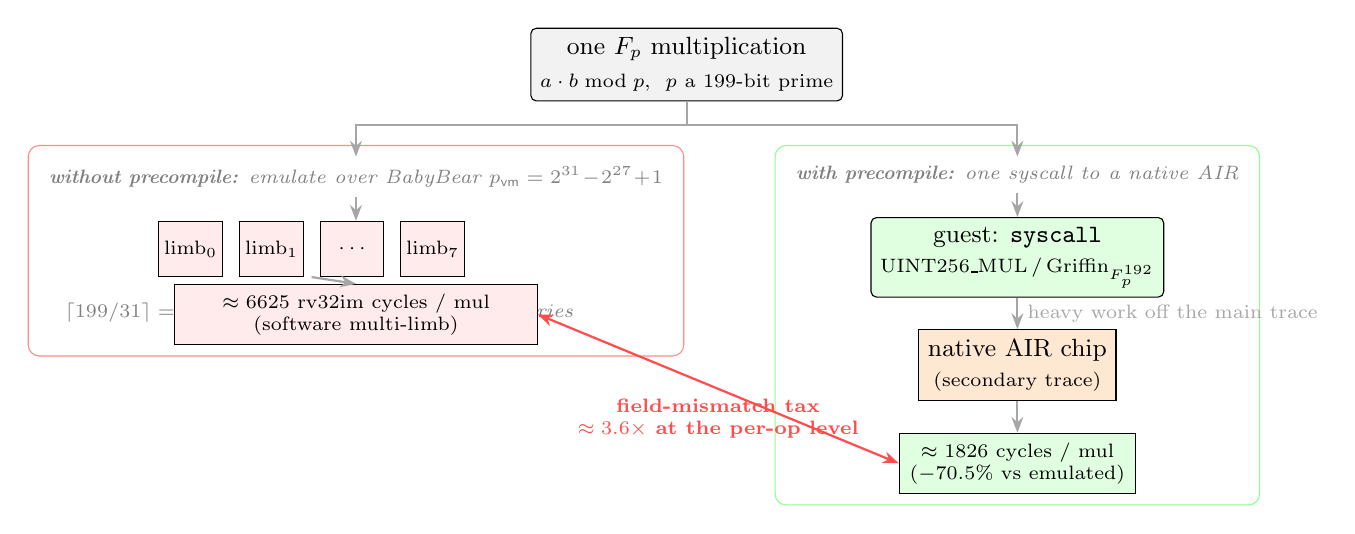
\begin{tikzpicture}[
  font=\small,>={Stealth[length=2mm]},
  op/.style={draw,rounded corners=2pt,fill=gray!10,minimum width=30mm,minimum height=8mm,align=center},
  emu/.style={draw,fill=red!8,minimum width=8mm,minimum height=7mm,inner sep=2pt,font=\scriptsize,align=center},
  pre/.style={draw,rounded corners=2pt,fill=green!12,minimum width=30mm,minimum height=8mm,align=center},
  chip/.style={draw,fill=orange!18,minimum width=24mm,minimum height=8mm,align=center},
  lbl/.style={font=\scriptsize\itshape,gray},
  flow/.style={->,thick,gray!70},
]

% top: the source operation
\node[op] (src) {one $\mathbb{F}_p$ multiplication\\[1pt]\scriptsize $a\cdot b \bmod p$,\ \ $p$ a $199$-bit prime};

% ===== LEFT PATH: emulation over BabyBear =====
\node[lbl,below=7mm of src,xshift=-42mm] (emuhdr) {\textbf{without precompile:} emulate over BabyBear $p_{\mathsf{vm}}=2^{31}\!-\!2^{27}\!+\!1$};
\node[emu,below=3mm of emuhdr,xshift=-21mm] (l0) {limb$_0$};
\node[emu,right=2mm of l0] (l1) {limb$_1$};
\node[emu,right=2mm of l1] (l2) {$\cdots$};
\node[emu,right=2mm of l2] (l3) {limb$_7$};
\node[lbl,below=2mm of l1,xshift=6mm] {$\lceil 199/31\rceil=7$ limbs; $7\times7$ partial products\,+\,carries};
\node[draw,fill=red!8,below=11mm of emuhdr,minimum width=46mm,minimum height=7mm,align=center,font=\scriptsize] (emucost)
   {$\approx 6625$ rv32im cycles / mul\\(software multi-limb)};

% ===== RIGHT PATH: precompile =====
\node[lbl,below=7mm of src,xshift=42mm] (prehdr) {\textbf{with precompile:} one syscall to a native AIR};
\node[pre,below=3mm of prehdr] (sys) {guest: \texttt{syscall}\\\scriptsize UINT256\_MUL\,/\,Griffin$_{\mathbb{F}_p^{192}}$};
\node[chip,below=4mm of sys] (air) {native AIR chip\\\scriptsize (secondary trace)};
\node[draw,fill=green!12,below=4mm of air,minimum width=30mm,minimum height=7mm,align=center,font=\scriptsize] (precost)
   {$\approx 1826$ cycles / mul\\($-70.5\%$ vs emulated)};

% arrows
\draw[flow] (src.south) -- ++(0,-3mm) -| (emuhdr.north);
\draw[flow] (src.south) -- ++(0,-3mm) -| (prehdr.north);
\draw[flow] (emuhdr) -- (l1.north-|emuhdr);
\draw[flow] ($(l0.south)!0.5!(l3.south)$) -- (emucost.north);
\draw[flow] (prehdr) -- (sys);
\draw[flow] (sys) -- node[right,font=\scriptsize]{heavy work off the main trace} (air);
\draw[flow] (air) -- (precost);

% the "tax" bracket
\draw[<->,red!70,thick] (emucost.east) -- node[below,font=\scriptsize\bfseries,red!70,align=center]{field-mismatch tax\\$\approx 3.6\times$ at the per-op level} (precost.west);

\begin{scope}[on background layer]
  \node[fit=(emuhdr)(l0)(l3)(emucost),draw=red!45,rounded corners,inner sep=4pt]{};
  \node[fit=(prehdr)(sys)(air)(precost),draw=green!45,rounded corners,inner sep=4pt]{};
\end{scope}
\end{tikzpicture}
\end{document}
